%
% Sætning 6.2.7 (Cauchy-Schwarz Uligheden) side 101
%

\begin{saetning}{6.2.7 (Cauchy-Swartz-Uligheden)}
	Lad $V$ være et $\mathbb{R}$ eller $\mathbb{C}$ vektorrum med indre produkt
	$\langle$ , $\rangle$. Lad $\vec{u}, \vec{v} \in V$. Der gælder
	\[
		\lvert \langle \vec{u}, \vec{v} \rangle \rvert \leq \norm{\vec{u}}\norm{
		\vec{v}}
	\]
	Ligheden gælder hvis og kun hvis $\vec{u}$, $\vec{v}$ er lineært afhængige.
\end{saetning}

\begin{bevis}
	Hvis $\vec{v}=\vec{0}$ er der lighed
	\[
		\lvert \langle \vec{u}, \vec{v} \rangle \rvert = 0 = \norm{\vec{u}}
		\norm{\vec{v}}
	\]
	
	\noindent Hvis $\vec{v} \not= \vec{0}$ lades $\vec{p}$ være projektionen af $\vec{u}$
	på $\vec{v}$. Da $\vec{p}$ og $\vec{u} - \vec{p}$ er ortogonale er
	\[
		\norm{\vec{p}}^2 + \norm{\vec{u} - \vec{p}}^2 = \norm{\vec{u}}^2
	\]
	Fra skalarprojektionen så
	\[
		\frac{\lvert \langle \vec{u}, \vec{v} \rangle \rvert^2}{\norm{\vec{v}}^2}
		= {\lvert \alpha \rvert}^2 = \alpha \overline\alpha = \norm{\vec{p}}^2
		= \norm{\vec{u}}^2 - \norm{\vec{u} - \vec{p}}^2
	\]
	\begin{center}
		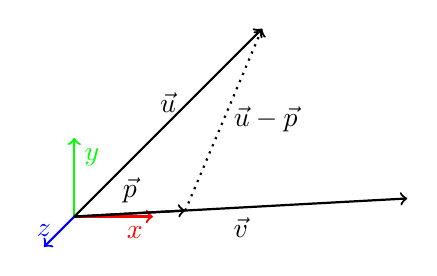
\begin{tikzpicture}
			\coordinate (0) at (0,0,0);
			\coordinate (v) at (5,1,2);
			\coordinate (u) at (2,2,-1);
			\coordinate (p) at (5/3,1/3,2/3);

			\draw[thick,->,color=red] (0,0,0) -- (1,0,0) node[anchor=north east]{$x$};
			\draw[thick,->,color=green] (0,0,0) -- (0,1,0) node[anchor=north west]{$y$};
			\draw[thick,->,color=blue] (0,0,0) -- (0,0,1) node[anchor=south]{$z$};
			
			\draw[thick,->] (0) to node[below]{$\vec{v}$} (v);
			\draw[thick,->] (0) to node[above]{$\vec{u}$} (u);
			\draw[thick,->] (0) to node[above]{$\vec{p}$} (p);
			\draw[thick,->,dotted] (p) to node[right]{$\vec{u}-\vec{p}$} (u);
		\end{tikzpicture}
	\end{center}
	Hvilket giver
	\[
		\lvert \langle \vec{u}, \vec{v} \rangle \rvert^2 = \norm{\vec{u}}^2
		\norm{\vec{v}}^2 - \norm{\vec{u} - \vec{p}}^2\norm{\vec{v}}^2 \leq
		\norm{\vec{u}}^2\norm{\vec{v}}^2
	\]
	hvor der gælder lighed hvis $u=p$.

	Det er hermed vist at der kun gælder lighed når $u$ og $v$ er lineært
	afhængige.
\end{bevis}
